% Déclaration du type de document (report, book, paper, etc...)
\documentclass[a4paper, 12pt]{paper} 
 
% Package pour avoir Latex en français
\usepackage[utf8]{inputenc}
\usepackage[T1]{fontenc}
 
% Quelques packages utiles
\usepackage{listings} % Pour afficher des listings de programmes
\usepackage{graphicx} % Pour afficher des figures
\usepackage{amsthm}   % Pour créer des théorèmes et des définitions
\usepackage{amsmath}
\usepackage{microtype} % Optical margins FTW
\usepackage{url}
\usepackage{booktabs} % Allows the use of \toprule, \midrule and \bottomrule in tables for horizontal lines
\usepackage[per-mode=symbol]{siunitx}
\usepackage{floatrow}
\usepackage{caption}
\usepackage{subcaption}
\usepackage{fullpage}
\usepackage{lipsum}



\author{Loïc Amez-Droz \and Florian Reinhard}
\title{Monomode Fiber}

% Début du document
\begin{document}
\begin{titlepage}
\begin{center}
    \textsc{\LARGE École Polytechnique Fédérale de~Lausanne}\\[1.5cm] 
    {\huge \bfseries Optical Engineering: Multimode Fibre}\\[0.4cm] 
    \begin{tabular}{|p{5cm}|p{4cm}|}
        \hline
        Group & C-XX \\ \hline
        Students & Loïc \textsc{Amez-Droz} \newline Florian \textsc{Reinhard} \\ \hline
        Date of lecture & 13.03.2015 \\ \hline
        Date of final report return & 20.03.2015 \\ \hline
    \end{tabular}
\end{center}


\begin{abstract}
    \lipsum[3]
\end{abstract}
 
\vfill
\end{titlepage}

\section{Procedures and results}
\subsection{Monomode optical fiber injection and mode profiles}

We observe the behavior of a laser source through a monomode fiber.
Moving the 6 axis positioning system of the fiber entrance and the source, we try to find different modes.
The fiber used is the \emph{P1-SMF28E-FC-2} $\left( \lambda \approx \SI{1.5}{\micro\meter} \right)$.

\begin{figure}[H]
    \centering
    \begin{subfigure}[t]{0.3\textwidth}
        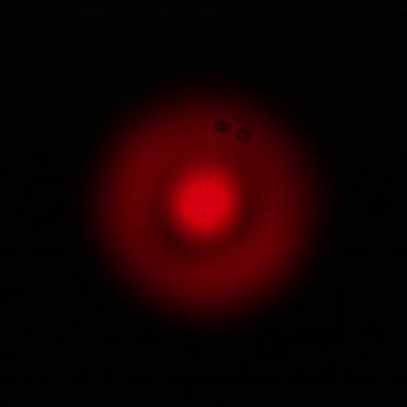
\includegraphics[width=\textwidth]{img/mode_2}
        \caption{$LP_{0}$.}
    \end{subfigure}
    \begin{subfigure}[t]{0.3\textwidth}
        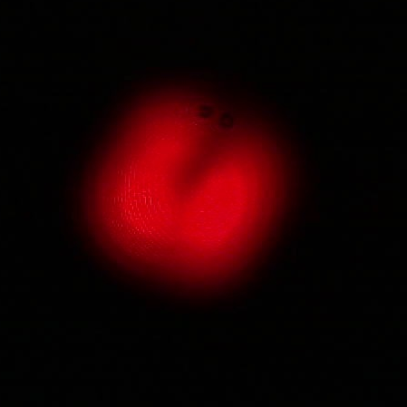
\includegraphics[width=\textwidth]{img/mode_3}
        \caption{$LP_{1}$.}
    \end{subfigure}
    \begin{subfigure}[t]{0.3\textwidth}
        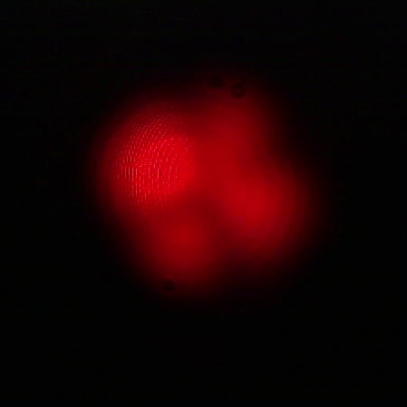
\includegraphics[width=\textwidth]{img/mode_1}
        \caption{$LP_{2}$.}
\label{fig:mode_1}
    \end{subfigure}
    \caption{Spots resulting from different modes in the fiber.}
\label{fig:modes}
\end{figure}

The wavelength of the laser (\SI{633}{\nano\meter}) being smaller than the fiber one we can observe different vibration modes.
The image contrasts are caused by the constructive respectively destructive interferences. 
In the second part we observe the intensity distribution using a polarizer in two different positions (figure~\ref{fig:polarizer}).

\begin{figure}[H]
    \centering
    \begin{subfigure}[t]{0.3\textwidth}
        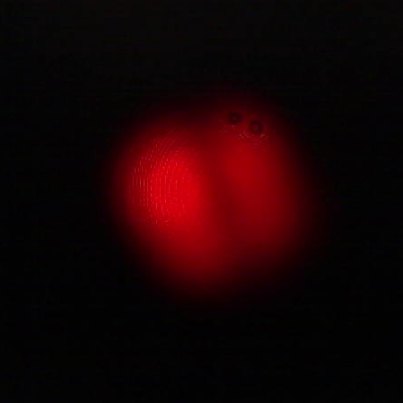
\includegraphics[width=\textwidth]{img/polarizer_0}
        \caption{Polarizer at \SI{0}{\degree}}
    \end{subfigure}
    \begin{subfigure}[t]{0.3\textwidth}
        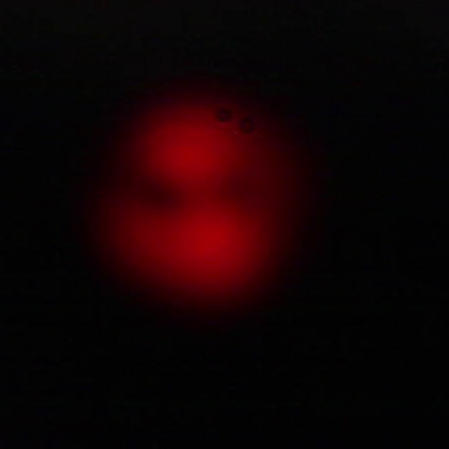
\includegraphics[width=\textwidth]{img/polarizer_90}
        \caption{Polarizer at \SI{90}{\degree}}
    \end{subfigure}
    \caption{Rotating the polarizer in front of the source a quarter-turn, we can observe two orthogonal modes.
        Together they form a mode like in figure~\ref{fig:mode_1}.}
\label{fig:polarizer}
\end{figure}

\subsection{Numerical aperture measurement}

\begin{figure}[H]
    \centering
    \begin{subfigure}[t]{0.5\textwidth}
        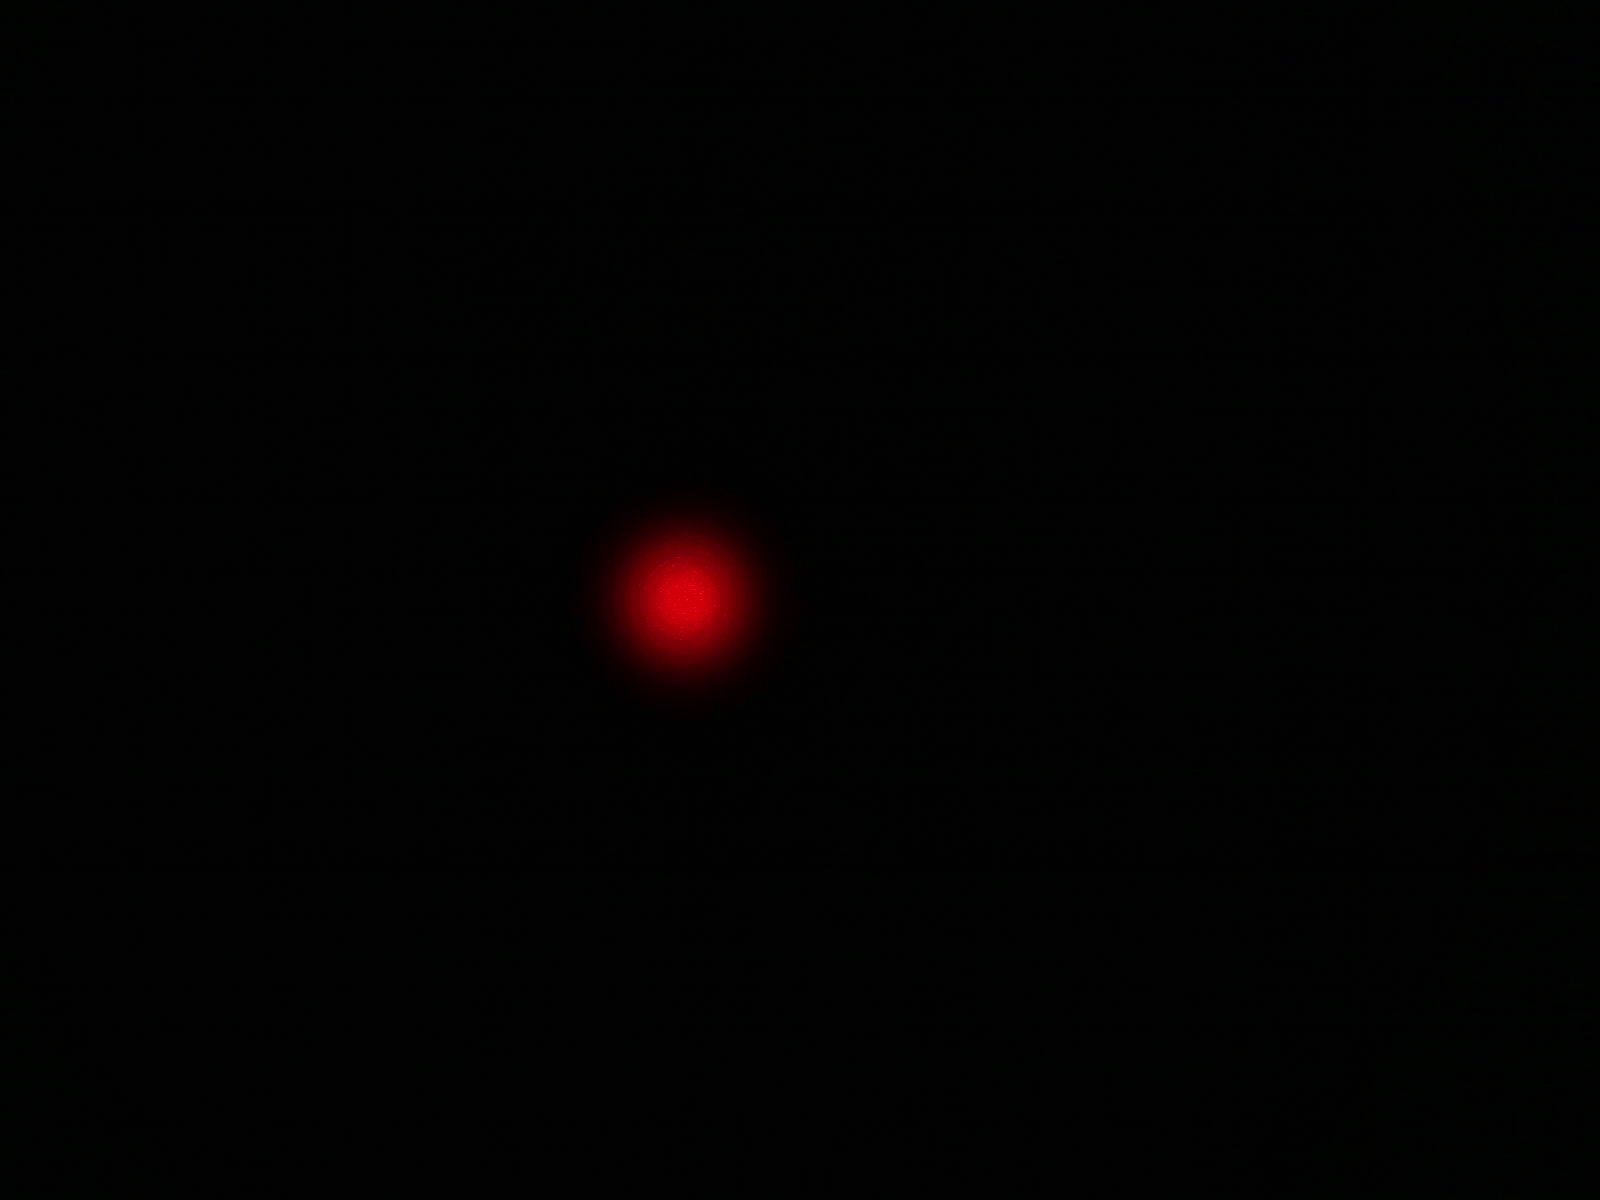
\includegraphics[width=\textwidth]{img/0mm.jpg}
        \caption{\SI{0}{\milli\meter}}
    \end{subfigure}
    \begin{subfigure}[t]{0.4\textwidth}
        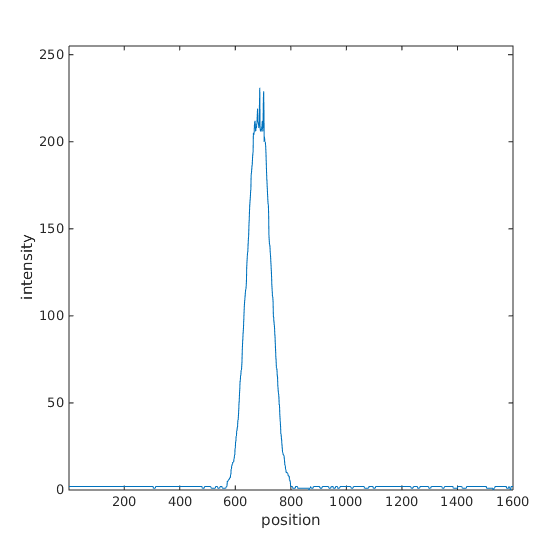
\includegraphics[width=\textwidth]{img/0mm_line}
        \caption{237px spot diameter}
    \end{subfigure}
    \begin{subfigure}[t]{0.5\textwidth}
        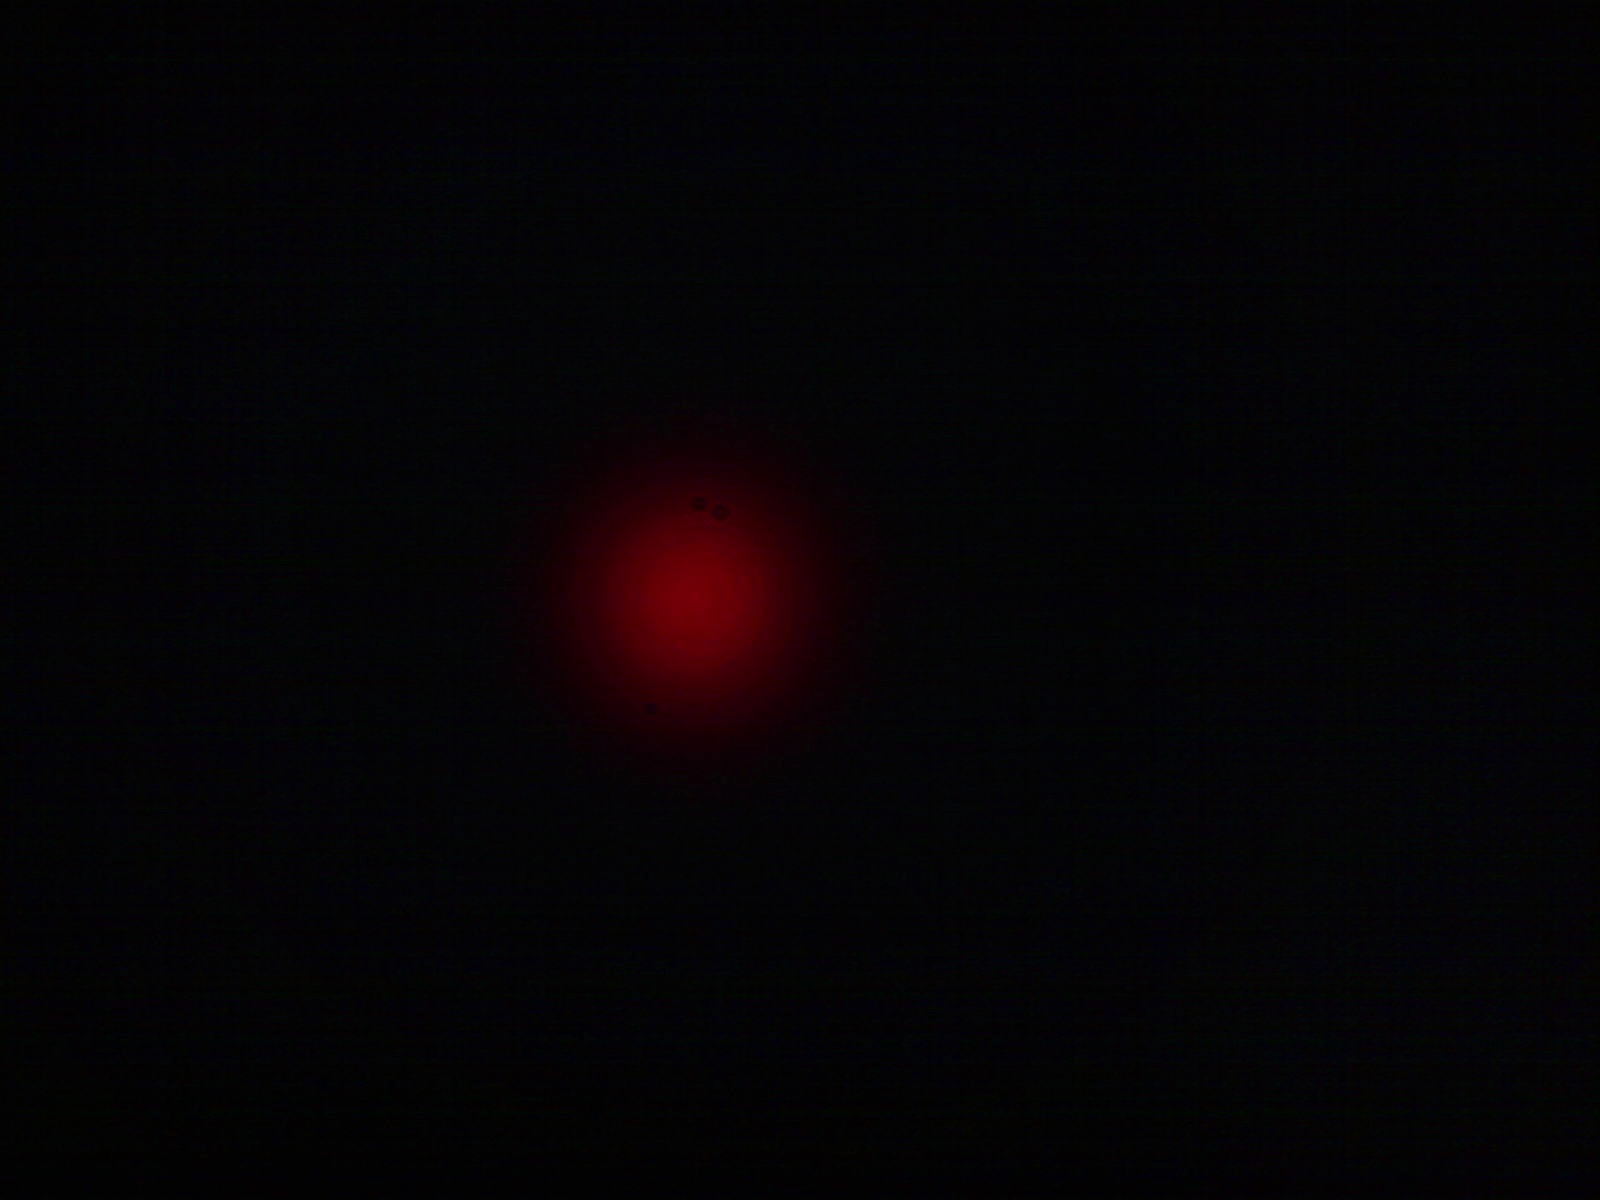
\includegraphics[width=\textwidth]{img/2mm.jpg}
        \caption{\SI{2}{\milli\meter}}
    \end{subfigure}
    \begin{subfigure}[t]{0.4\textwidth}
        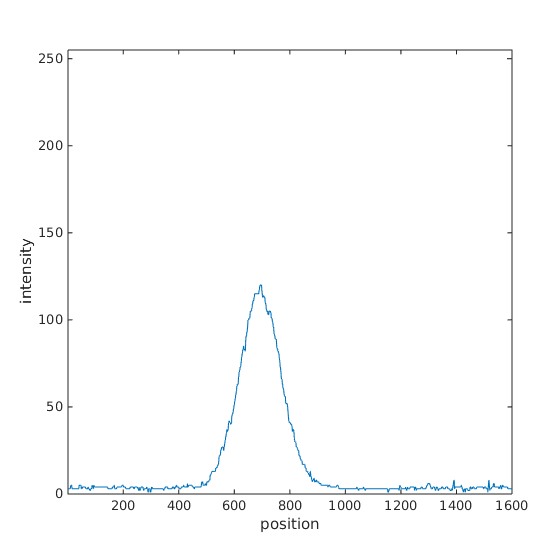
\includegraphics[width=\textwidth]{img/2mm_line}
        \caption{410px spot diameter}
    \end{subfigure}
    \begin{subfigure}[t]{0.5\textwidth}
        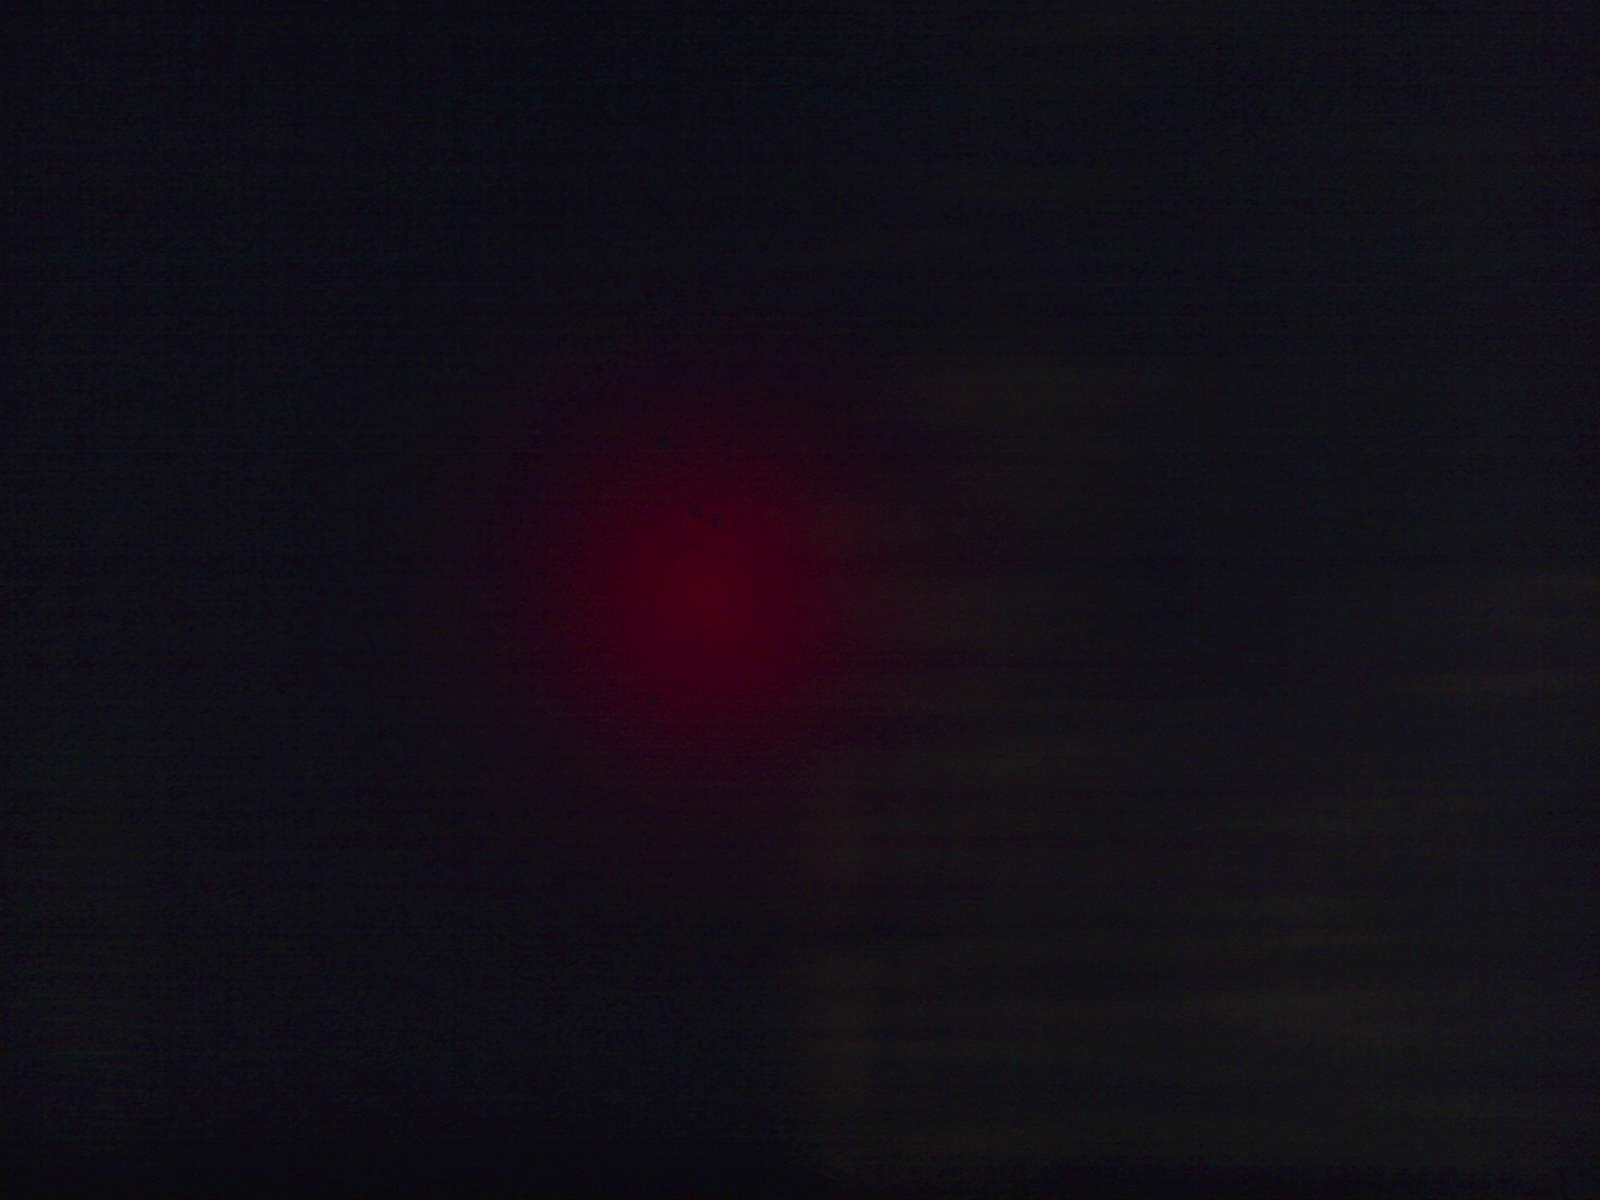
\includegraphics[width=\textwidth]{img/5mm.jpg}
        \caption{\SI{5}{\milli\meter}}
    \end{subfigure}
    \begin{subfigure}[t]{0.4\textwidth}
        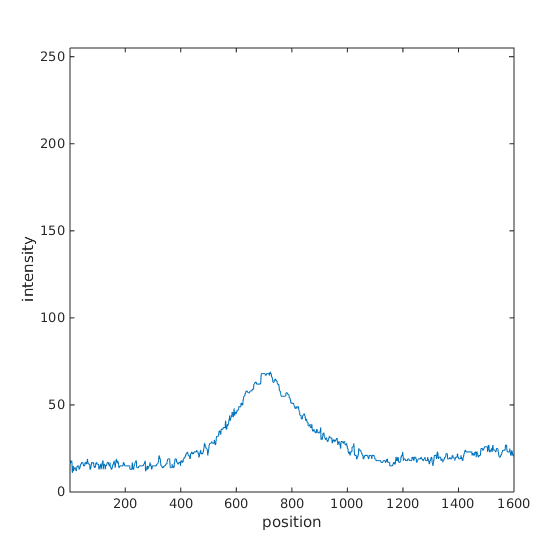
\includegraphics[width=\textwidth]{img/5mm_line}
        \caption{690px spot diameter}
\label{fig:5mm}
    \end{subfigure}
    \caption{Spot diameters with the fiber exit at different distances from the sensor.
        The size of one pixel is \SI{2.835}{\micro\meter}.}
\label{fig:spot_diams}
\end{figure}

\begin{table}[H]
    \centering
    \begin{tabular}{S[table-format=1.2] S[table-format=3.0] S[table-format=1.3]}
        \toprule
        {Distance from fiber exit to sensor (\SI{}{\milli\meter})} & {Spot diameter (px)} & {(\SI{}{\milli\meter})} \\
        \midrule
        0.00 & 237 & 0.6719 \\ 
        1.00 & 340 & 0.9639 \\
        2.00 & 410 & 1.1623 \\
        3.00 & 486 & 1.3778 \\
        4.00 & 551 & 1.5621 \\
        5.00 & 690 & 1.9561 \\
        \bottomrule
    \end{tabular}
    \caption{Spot sizes at different positions relative to the fiber exit as measured in figure~\ref{fig:spot_diams}.}
\label{tab:injection_ratios}
\end{table}

\begin{figure}[H]
    \centering
    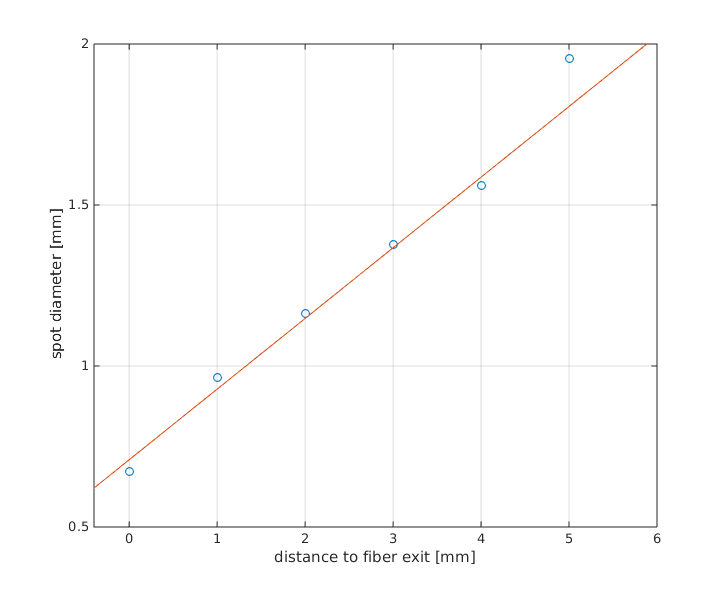
\includegraphics[width=0.7\textwidth]{img/diameter_graph}
    \caption{Spot sizes in relation to the distance to the sensor with a line fitted to them.
        The measurement at \SI{5}{\milli\meter} is considered to be an out-runner, as it is quite noisy (figure~\ref{fig:5mm}).
        The line's slope of 0.22 is $ 2 \times \sin{\theta} $ with $\theta$ being half the angle of the maximum angle exiting the fiber.}
\label{fig:diameter_graph}
\end{figure}

\begin{equation}
    \mbox{NA} = n \sin \theta = 0.11
    \label{equ:NA}
\end{equation}

The \emph{root mean square} of the difference of the measurements in figure~\ref{fig:diameter_graph} to the fitted line is $\sigma = \SI{0.012}{\milli\meter}$, which yeilds $\frac{\Delta \mbox{NA}}{\mbox{NA}} = \SI{5.4}{\percent}$. 


\subsection{Coupling for different numerical apertures}

\begin{figure}[H]
    \centering
    \begin{subfigure}[t]{0.40\textwidth}
        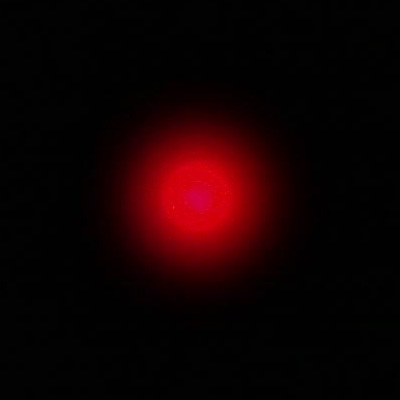
\includegraphics[width=\textwidth]{img/first.jpg}
        \caption{Low NA.}
    \end{subfigure}
    \begin{subfigure}[t]{0.45\textwidth}
        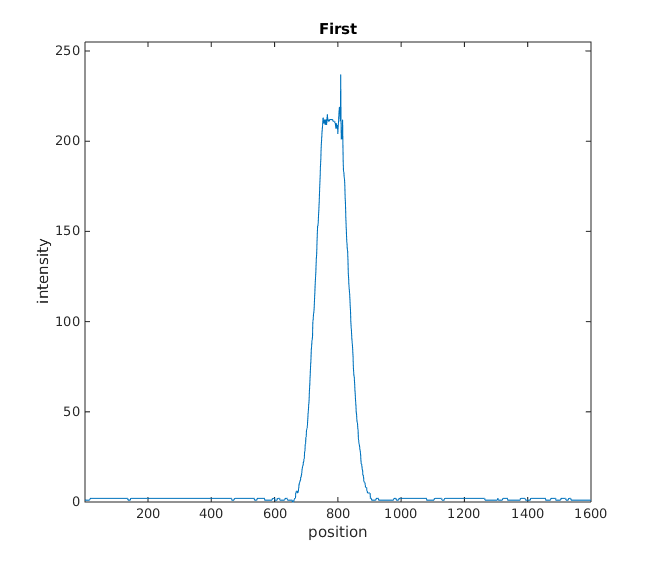
\includegraphics[width=\textwidth]{img/first_line}
        \caption{Line plot for low NA.}
    \end{subfigure}
    \begin{subfigure}[t]{0.40\textwidth}
        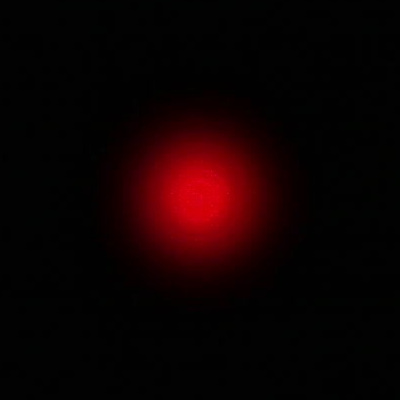
\includegraphics[width=\textwidth]{img/second.jpg}
        \caption{High NA.}
    \end{subfigure}
    \begin{subfigure}[t]{0.45\textwidth}
        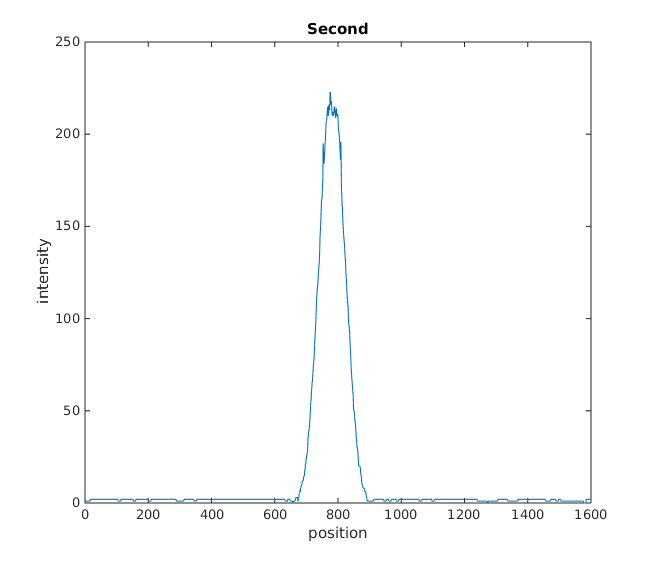
\includegraphics[width=\textwidth]{img/second_line}
        \caption{Line plot for high NA.}
    \end{subfigure}
    \caption{Spots and their line plots with the source at different distances from the fiber entrance and thus different numerical apertures.}
\label{fig:different_NAs}
\end{figure}


\begin{figure}[H]
    \centering
    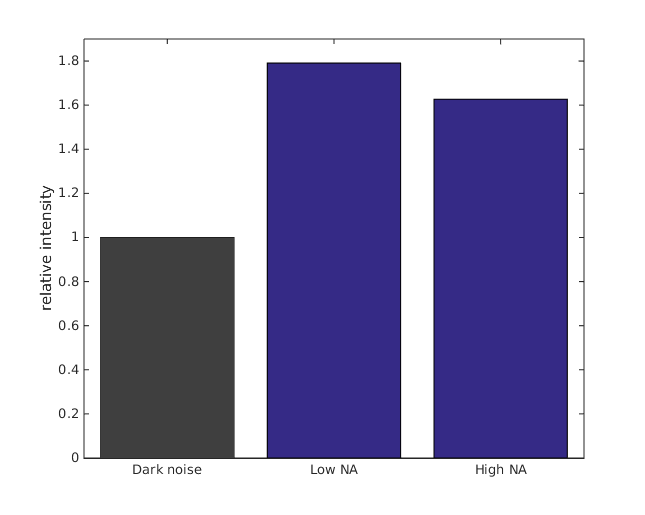
\includegraphics[width=0.8\textwidth]{img/NA_intensities}
    \caption{Relative intensities with different numerical apertures at the entrance of the fiber.}
\label{fig:NA_intensities}
\end{figure}

The figure~\ref{fig:NA_intensities} suggests that the coupling with the lower numerical aperture is more efficient.
This is probably because the lower NA is better adapted to the fiber's acceptance angle.

\subsection{Monomode fiber coupling for different sources}

To compare the coupling of different sources we use the fiber \emph{P1-630A-FC} $\left( \lambda = \SI{633}{\nano\meter} \right)$ and a planoconvex lens.
It is a monomode fiber for these sources.

The laser source is the easiest to be coupled into the \emph{P1-630A-FC} fiber.
The laser $\left( \lambda = \SI{633}{\nano\meter} \right)$ has the ideal wavelength and is a coherent source.
The coupling is worse with the halogen source, which is an incoherent one.
So the closed wavelengths tend to cancel.
The fiber's cut-off wavelength is $550 \pm \SI{50}{\nano\meter}$.
Thus the light is badly transmitted below \SI{500}{\nano\meter}, multimode to \SI{633}{\nano\meter} and monomode after. 
The coupling with the LED is really dark.
Due to its incoherence, the wavelengths close to each other cancel out.
The spectrum is narrower than the halogen source's one.

\begin{figure}[H]
    \centering
    \begin{subfigure}[t]{0.3\textwidth}
        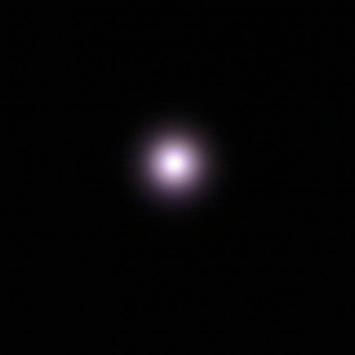
\includegraphics[width=\textwidth]{img/halogen_spot}
        \caption{Coupling the halogen source.}
    \end{subfigure}
    \begin{subfigure}[t]{0.3\textwidth}
        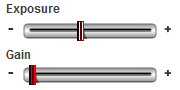
\includegraphics[width=\textwidth]{img/halogen}
    \end{subfigure}


    \begin{subfigure}[t]{0.3\textwidth}
        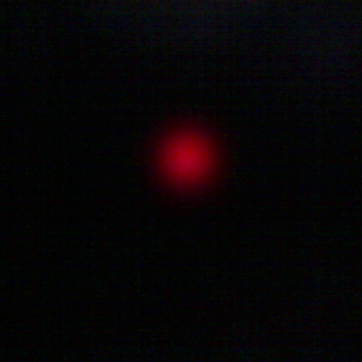
\includegraphics[width=\textwidth]{img/LED_spot}
        \caption{Coupling the LED source.}
    \end{subfigure}
    \begin{subfigure}[t]{0.3\textwidth}
        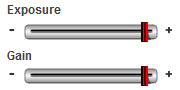
\includegraphics[width=\textwidth]{img/LED}
    \end{subfigure}


    \begin{subfigure}[t]{0.3\textwidth}
        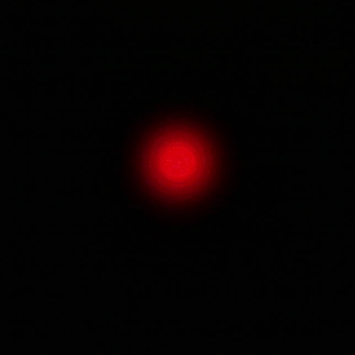
\includegraphics[width=\textwidth]{img/laser_spot}
        \caption{Coupling the laser source.}
    \end{subfigure}
    \begin{subfigure}[t]{0.3\textwidth}
        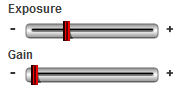
\includegraphics[width=\textwidth]{img/laser}
    \end{subfigure}
    \caption{Comparison of different light sources being coupled into an optical fiber.}
\label{fig:different_sources}
\end{figure}

\section{Discussion and conclusions}

We learned that wavelength and numerical aperture of the source are important for an optimal coupling with optical fibers.
It is difficult to couple incoherent light into a fiber.
When there are several modes in a fiber, then they are very unstable and prone to perturbations, such as movements of the fiber, changes in polarization of the source, and position as well as orientiation of the source in relation the the fiber's entrance.


\end{document}
